%%%%%%%%%%%%%%%%%%%%%%%%%%%%%%%%%%%%%%%%%%%%%%%%%%%%%%%%%%%%%%%%%%% 
%%%%%%%%%%%%%%%%%%%%%%%%%%%%%%%%%%%%%%%%%%%%%%%%%%%%%%%%%%%%%%%%%%% 
%%%%%%%%%%%%%%%%%%%%%%%%%%%%%%%%%%%%%%%%%%%%%%%%%%%%%%%%%%%%%%%%%%% 
\begin{frame}
  \frametitle{Kokkos Concepts (1) - the abstract machine model}

  \begin{itemize}
  \item Kokkos defines an abstract machine model for future large shared-memory nodes made of 
    \begin{itemize}
    \item \textcolor{blue}{\textbf{latency-oriented cores}} (contemporary CPU core)
    \item \textcolor{orange}{\textbf{throughput-oriented cores}} (GPU, ...)
    \end{itemize}
  \end{itemize}

  \begin{center}
    \begin{figure}
      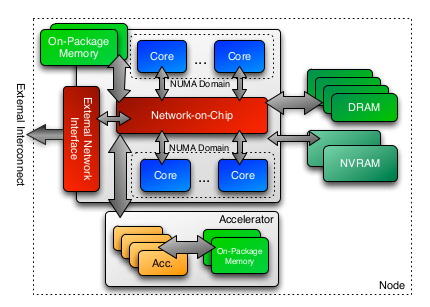
\includegraphics[width=5cm]{images/kokkos_machine_model}
      \caption{Conceptual model of a future HPC node. (Kokkos User's Guide).}
      \end{figure}
  \end{center}

\end{frame}


%%%%%%%%%%%%%%%%%%%%%%%%%%%%%%%%%%%%%%%%%%%%%%%%%%%%%%%%%%%%%%%%%%% 
%%%%%%%%%%%%%%%%%%%%%%%%%%%%%%%%%%%%%%%%%%%%%%%%%%%%%%%%%%%%%%%%%%% 
%%%%%%%%%%%%%%%%%%%%%%%%%%%%%%%%%%%%%%%%%%%%%%%%%%%%%%%%%%%%%%%%%%% 
\begin{frame}[fragile=singleslide]
  \frametitle{Kokkos Concepts (2) - What is a device ?}

  \begin{itemize}
  \item A \textcolor{red}{\textbf{Kokkos device}}: 
  \item From a C++ API design point of view, Kokkos defines several c++ class for a \textcolor{red}{device} in \texttt{core/src}, e.g.
    \begin{itemize}
    \item Kokkos::Cuda, Kokkos::OpenMP, Kokkos::Pthreads, Kokkos::Serial
    \item \textcolor{blue}{\textit{device} = execution space + memory space}
    \end{itemize}
  \item Each \textit{Kokkos device} pre-defines some types
  \item Example \textcolor{red}{\textbf{Kokkos device}} (not required for a user, only Kokkos developper), e.g.\\
    {\tiny
      \begin{minted}{c++}
        class Cuda {
          public:
          // Tag this class as a kokkos execution space
          typedef Cuda                  execution_space ;
          
          #if defined( KOKKOS_USE_CUDA_UVM )
          // This execution space's preferred memory space.
          typedef CudaUVMSpace          memory_space ;
          #else
          // This execution space's preferred memory space.
          typedef CudaSpace             memory_space ;
          #endif
          
          // This execution space preferred device_type
          typedef Kokkos::Device<execution_space,memory_space> device_type;
          
          // The size_type best suited for this execution space.
          typedef memory_space::size_type  size_type ;
          
          // This execution space's preferred array layout.
          typedef LayoutLeft            array_layout ;
          ...
        } // end class Cuda
        \end{minted}
      }
  \end{itemize}

\end{frame}

%%%%%%%%%%%%%%%%%%%%%%%%%%%%%%%%%%%%%%%%%%%%%%%%%%%%%%%%%%%%%%%%%%% 
%%%%%%%%%%%%%%%%%%%%%%%%%%%%%%%%%%%%%%%%%%%%%%%%%%%%%%%%%%%%%%%%%%% 
%%%%%%%%%%%%%%%%%%%%%%%%%%%%%%%%%%%%%%%%%%%%%%%%%%%%%%%%%%%%%%%%%%% 
\begin{frame}
  \frametitle{Kokkos Concepts (3) - execution space, memory space}

  \begin{itemize}
  \item \textcolor{blue}{\textbf{Execution space:}} Where should a parallel contruct (\texttt{parallel\_for}, \texttt{parallel\_reduce}, ...) be executed\\
    \begin{itemize}
    \item Special case: \texttt{class HostSpace}, special device (always defined) where execution space is either (Serial, Pthread or OpenMP).
    \item Each execution space is equipped with a \texttt{fence}: \texttt{Kokkos::Cuda::fence()}
    \end{itemize}
  \item \textcolor{blue}{\textbf{Memory space:}} Where / how data are allocated in memory (HostSpace, CudaSpace, CudaUVMSpace, CudaHostPinnedSpace, HBWSpace, ...)
  \item \textcolor{blue}{\textbf{Memory layout}} (we will come back later on that)
  \item Other concepts:
    \begin{itemize}
    \item Execution policy: used to modify a parallel thread dispatch
    \end{itemize}
  \item \textcolor{red}{Multiple execution / memory space} can be used in a single application\\
    See for example in Kokkos sources \texttt{example/tutorial/Advanced\_View/07\_Overlapping\_DeepCopy}\\
    Though, take care that currently, Cuda stream are not completely mapped into Kokkos API~\footnote{To be implemented.}; meanwhile Cuda streams can be used directly (but looses portability); 
  \end{itemize}

\end{frame}

